\documentclass[sigconf,anonymous,nonacm]{acmart}
\settopmatter{printacmref=false}
\setcopyright{none}
\pagestyle{plain}
\AtBeginDocument{\providecommand\BibTeX{{\normalfont B\kern-0.5em{\scshape i\kern-0.25em b}\kern-0.8em\TeX}}}
\graphicspath{{images/}}

\begin{document}

\title{Sparse-Autoencoder Dissection of Emotion Features in Frozen Speech Encoders}
\author{Anonymous Author(s)}
\affiliation{\institution{Anonymous}\country{}}
\renewcommand{\shortauthors}{Anonymous}

\begin{abstract}
Linear probes tell us that emotion becomes \emph{readable} in the middle-to-late layers of frozen speech transformers --- but not \emph{which} internal features carry it, and not whether a probe is listening to \emph{how} something is said (acoustics) or \emph{what} is said (words). We open these models up with Sparse Autoencoders (SAEs): we train a TopK SAE on the per-frame activations of six frozen large encoders (HuBERT, WavLM, wav2vec2, w2v-BERT, MERT, Whisper) and read off the individual features it learns. The trick that makes this work is a lexicon-controlled corpus, CREMA-D (91 actors $\times$ 12 \emph{fixed} sentences $\times$ 6 emotions), plus a confound check that keeps a feature only if it tells us more about emotion than about the sentence or the speaker --- otherwise the SAE just rediscovers phonemes. Four findings follow: (i) emotion is \emph{organised} into clean features earlier (layers 2--7) than where a probe reads it best (layer 10); (ii) all six encoders share a common, speaker-invariant acoustic feature basis; (iii) the recovered signal is acoustic, not lexical; and (iv) on incongruent speech (EMIS), the ``lexical shortcut'' is a \emph{deep-layer} habit that only the ASR-trained encoders pick up, while Whisper stays grounded in the voice at every layer.
\end{abstract}
\keywords{speech emotion recognition, sparse autoencoders, interpretability, disentanglement, acoustic features}
\maketitle

\section{Why this study}
Self-supervised speech encoders sit on top of the speech-emotion leaderboards, but they were originally trained to transcribe words, so they carry a lot of linguistic information. That raises an uncomfortable question: when a probe reads emotion out of one of these models, is it hearing the \emph{tone of voice}, or is it quietly reading the \emph{words}? A model that leans on the words will fail exactly where we most need it --- sarcasm, accents, and languages where the lexicon is unfamiliar.

Standard probing cannot answer this. It tells us \emph{where} emotion is decodable, but treats the layer as a black box. We instead use a Sparse Autoencoder, which factors the dense activation of a layer into a large dictionary of sparse, mostly single-meaning ``features.'' Inspecting those features lets us ask \emph{which} ones track emotion, \emph{what} they respond to (prosody vs.\ words), and \emph{whether} they are shared across models and speakers. In short, we move from \textbf{decodability} to \textbf{mechanism}.

A known hazard is that an SAE trained on ordinary speech mostly rediscovers \emph{phonemes}~\cite{saeasr2026,pluth2026asrsae}. We sidestep it by anchoring on CREMA-D, where the 12 carrier sentences are identical across emotions, so a recovered emotion signal cannot be coming from the words. This doubles as a built-in sanity check.

\noindent\textbf{What we contribute.} (1) a confound-controlled recipe for finding genuine emotion features in speech SAEs; (2) the observation that disentanglement and decodability peak at \emph{different} depths; (3) an acoustic-vs-lexical label per feature plus a causal sufficiency test; and (4) a depth-resolved picture of the lexical shortcut on EMIS. Code and artifacts are released.

\section{How we did it}
\textbf{Activations.} The project's cached embeddings are averaged over time (one vector per clip), which is far too few examples to fit a large SAE. So we re-extract the \emph{un-pooled, per-frame} hidden states of all six frozen encoders --- 25 layers each (a CNN front-end plus 24 transformer layers), with Whisper's padding frames masked out. CREMA-D layer~13 alone gives $940{,}273$ frames to train on.

\noindent\textbf{The SAE.} A TopK SAE ($d_{\text{in}}{=}1024$, dictionary size $8192$, $k{=}32$ active features per frame), with a unit-norm decoder and a small auxiliary loss that keeps features from dying. It is a faithful compressor: it explains \textbf{93\%} of the activation variance with essentially no dead features (Table~\ref{tab:key}).

\noindent\textbf{Finding the emotion features --- and the confound check.} For every feature we measure how much its on/off firing tells us about the emotion label (mutual information, with a shuffle test for significance). The catch: at this scale almost everything is ``significant.'' What separates a real emotion feature from a phoneme detector is (a) \emph{monosemanticity} --- most of its activity falls on one emotion --- and (b) the \emph{confound check}: it must tell us more about emotion than about the spoken sentence (a stand-in for phonetics) \emph{or} the speaker. Significance plus monosemanticity alone flags 394 features, but two-thirds of those are really about the sentence or the speaker. After the confound check, \textbf{61} clean emotion features survive (Table~\ref{tab:key}); they are dominated by anger and sadness, while fear and neutral drop to zero --- exactly the high-arousal emotions that have the clearest acoustic signature.

\noindent\textbf{Acoustic or lexical?} For each emotion feature we ask whether its firing is better predicted by acoustic descriptors (eGeMAPS~\cite{eyben2016egemaps}) or by the sentence identity (the lexical content). We use classification AUC rather than $R^2$ because the features are about 96\% silent.

\begin{figure*}[t]
  \centering
  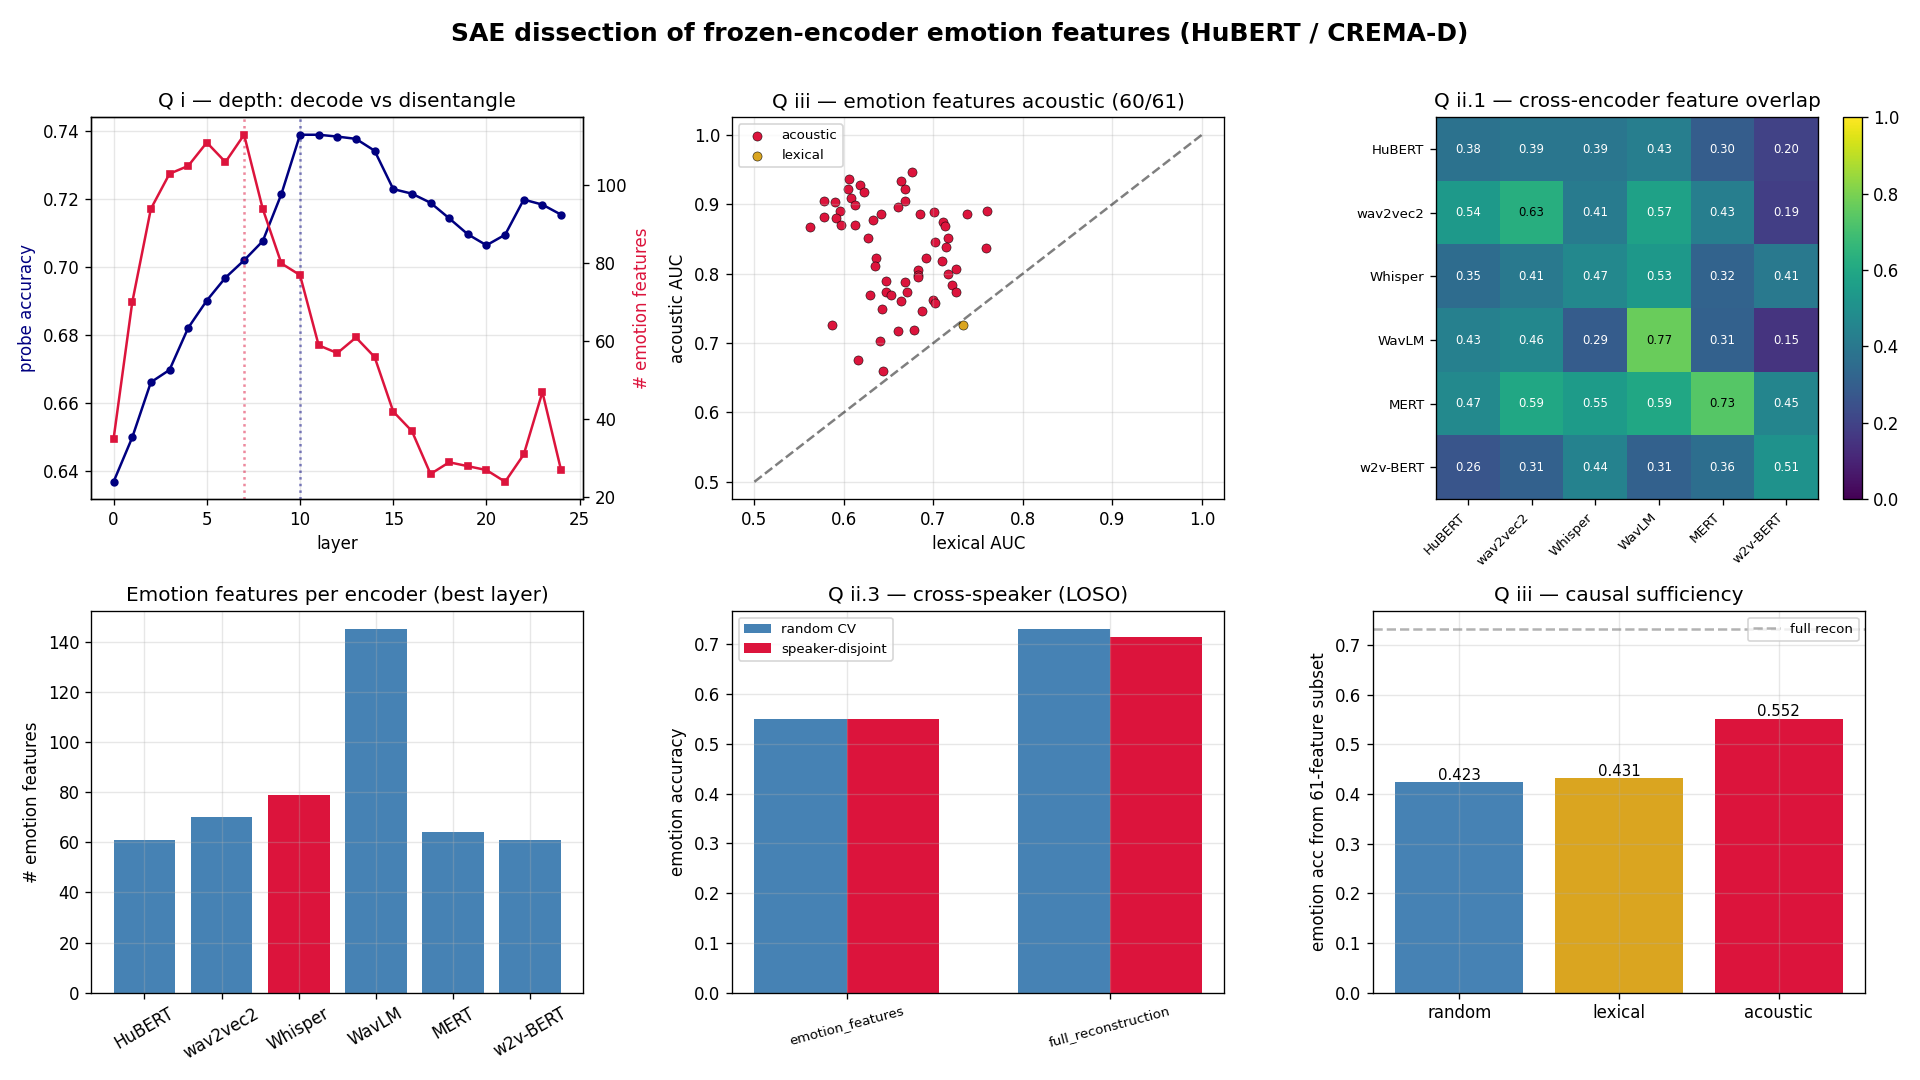
\includegraphics[width=0.9\textwidth]{fig_summary.png}
  \caption{The whole study at a glance (HuBERT / CREMA-D). \textbf{Top:} depth --- probe accuracy vs.\ number of clean emotion features per layer; each feature acoustic vs.\ lexical (above the line = acoustic); how features overlap across the six encoders. \textbf{Bottom:} number of emotion features per encoder; cross-speaker test (random vs.\ leave-speaker-out); and the causal test (how well emotion decodes from only-acoustic vs.\ only-lexical vs.\ random features).}
  \label{fig:summary}
\end{figure*}

\section{What we found}
\subsection{Emotion is organised earlier than it is decoded}
If you just train a probe, accuracy climbs and peaks \emph{deep} (layer 10) and stays high. But the \emph{clean} emotion features tell a different story: their count peaks \emph{early} (layer 7), and their purity even earlier (layer 2). By the deep layers, emotion is still easy to decode but has smeared out across many directions --- only 24--47 clean features remain (Fig.~\ref{fig:summary}, top-left; Fig.~\ref{fig:depthac}, left). In plain terms: \textbf{the model tidies emotion into neat features early, then a probe reads it best later, once it has been re-mixed for linear separability.} Decodability and disentanglement are not the same thing.

\subsection{The same acoustic features, across encoders and speakers}
Every encoder ends up with a healthy set of emotion features (Table~\ref{tab:encoders}), all anger/sadness-dominated. When we match features across encoders by how they fire, Whisper overlaps with the self-supervised models just as much as they overlap with each other (0.40 vs.\ 0.39). So on fixed-lexicon speech, \emph{Whisper is not special} --- its much-discussed difference is about text, which CREMA-D cannot expose (we return to it in \S\ref{sec:emis}). The features also travel across people: under a strict leave-one-speaker-out test over all 91 actors, accuracy barely moves (drop $\approx 0$) and each feature fires for $\sim$95\% of the actors who express its emotion. This also explains a known result elsewhere: the large speaker-out drop on MESD ($\sim$0.30) comes from \emph{speaker-entangled} features --- precisely the ones our confound check throws away.

\subsection{The signal is acoustic, not lexical}
On fixed-lexicon CREMA-D, an emotion feature \emph{must} be acoustic --- and 60 of 61 are (mean acoustic AUC 0.83 vs.\ 0.66 for sentence identity; Fig.~\ref{fig:summary}, top-middle). The causal test agrees: if we let emotion be decoded only from the acoustic features we get 0.55, but only from the lexical features just 0.43 --- barely above the 0.42 we get from random features (Fig.~\ref{fig:summary}, bottom-right). The acoustic features are \emph{sufficient}; the lexical ones are not.

\subsection{The lexical shortcut is a deep-layer habit}\label{sec:emis}
CREMA-D cannot test the text shortcut, because its text is fixed. EMIS~\cite{emis2025} can: it is synthetic speech where the \emph{written} emotion and the \emph{spoken} emotion are deliberately mismatched. We train a probe on the matched clips and test on the mismatched ones; ``text-bias'' is how often the model goes with the words instead of the voice. The result (Table~\ref{tab:emis}, Fig.~\ref{fig:emis}): every encoder is grounded in the voice early on, but the three ASR-trained self-supervised models (HuBERT, WavLM, wav2vec2) \emph{develop} the shortcut in their deep layers. Whisper never does --- it stays voice-grounded at every layer --- and the music model MERT and w2v-BERT never take it either. This reproduces the previously published per-encoder text-bias and adds the new part of the story: the shortcut lives at a depth Whisper simply never reaches.

\begin{figure*}[t]
  \centering
  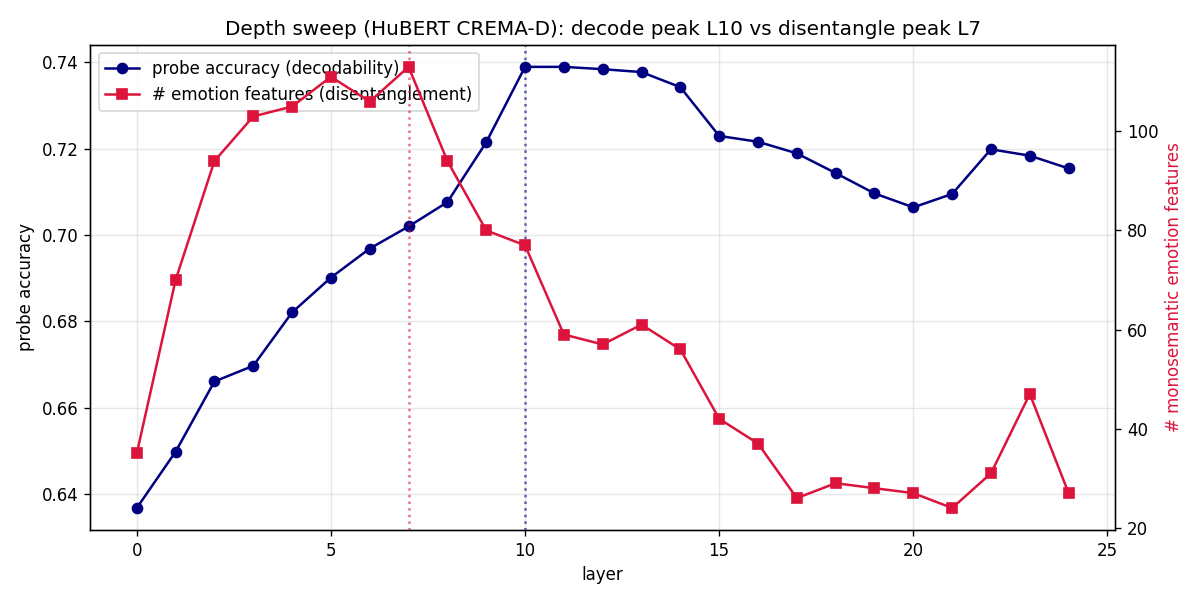
\includegraphics[height=2.25in]{fig_depth.png}\hspace{1.2em}
  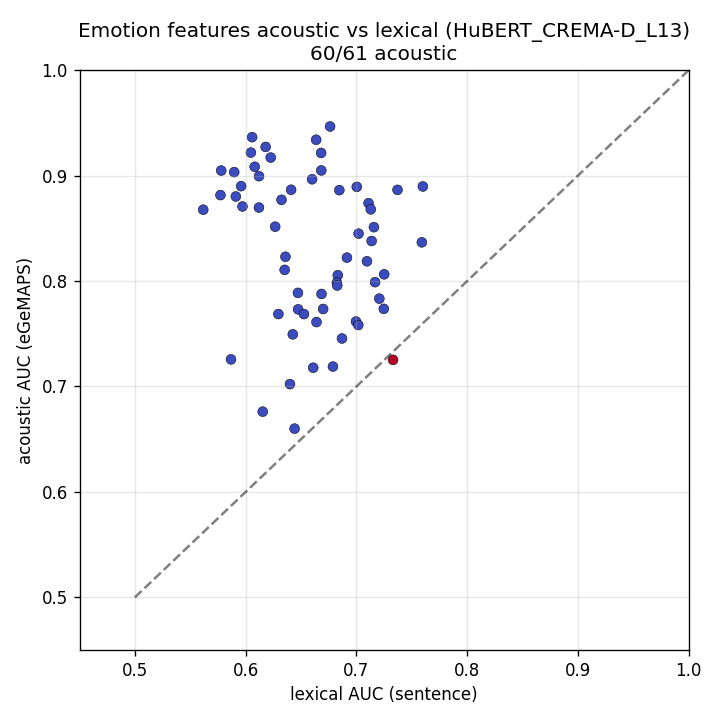
\includegraphics[height=2.25in]{fig_acoustic.png}
  \caption{\textbf{Left:} depth --- a probe reads emotion best deep (L10) while the count of clean emotion features peaks early (L7). \textbf{Right:} each emotion feature scored on acoustic (eGeMAPS) vs.\ lexical (sentence) prediction --- nearly all sit on the acoustic side of the diagonal.}
  \label{fig:depthac}
\end{figure*}

\begin{figure*}[t]
  \centering
  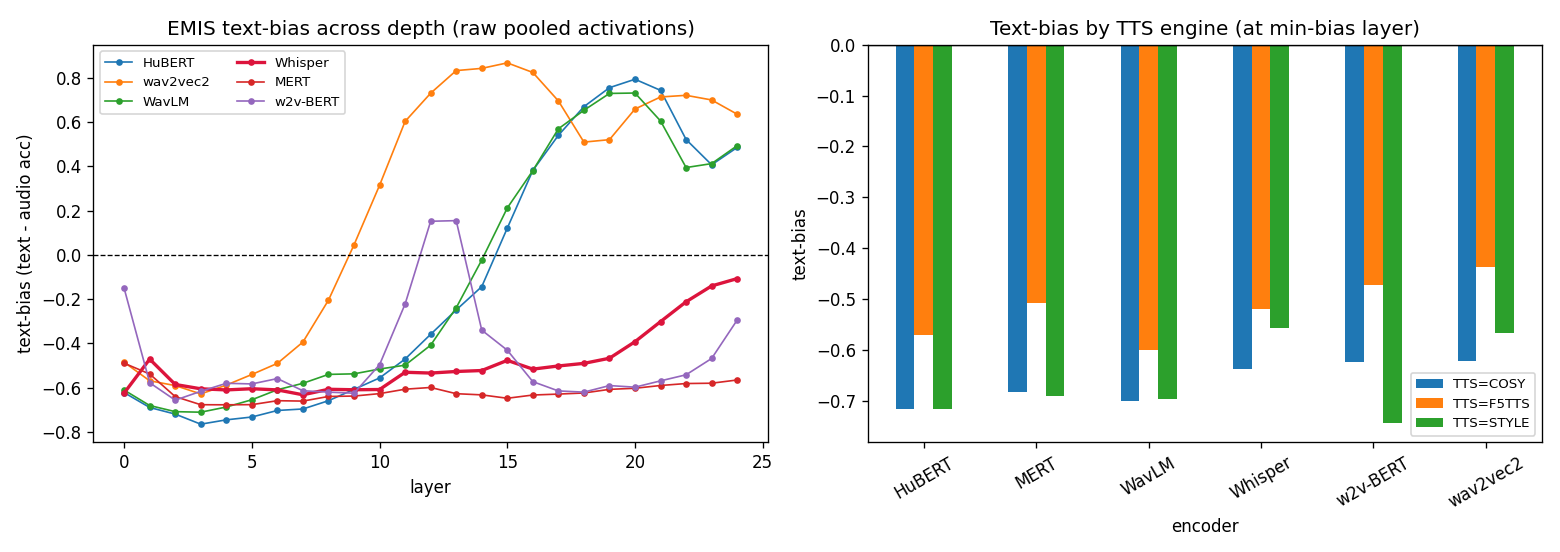
\includegraphics[width=0.96\textwidth]{fig_emis.png}
  \caption{EMIS text-bias (text $-$ audio accuracy) across all 25 layers. The ``use-the-words'' shortcut appears only in the \emph{deep} layers of the ASR-trained encoders (HuBERT/WavLM/wav2vec2); Whisper (red) stays voice-grounded at every layer, and MERT/w2v-BERT never take it. Right panel: the same broken down by TTS engine.}
  \label{fig:emis}
\end{figure*}

\begin{figure*}[t]
  \centering
  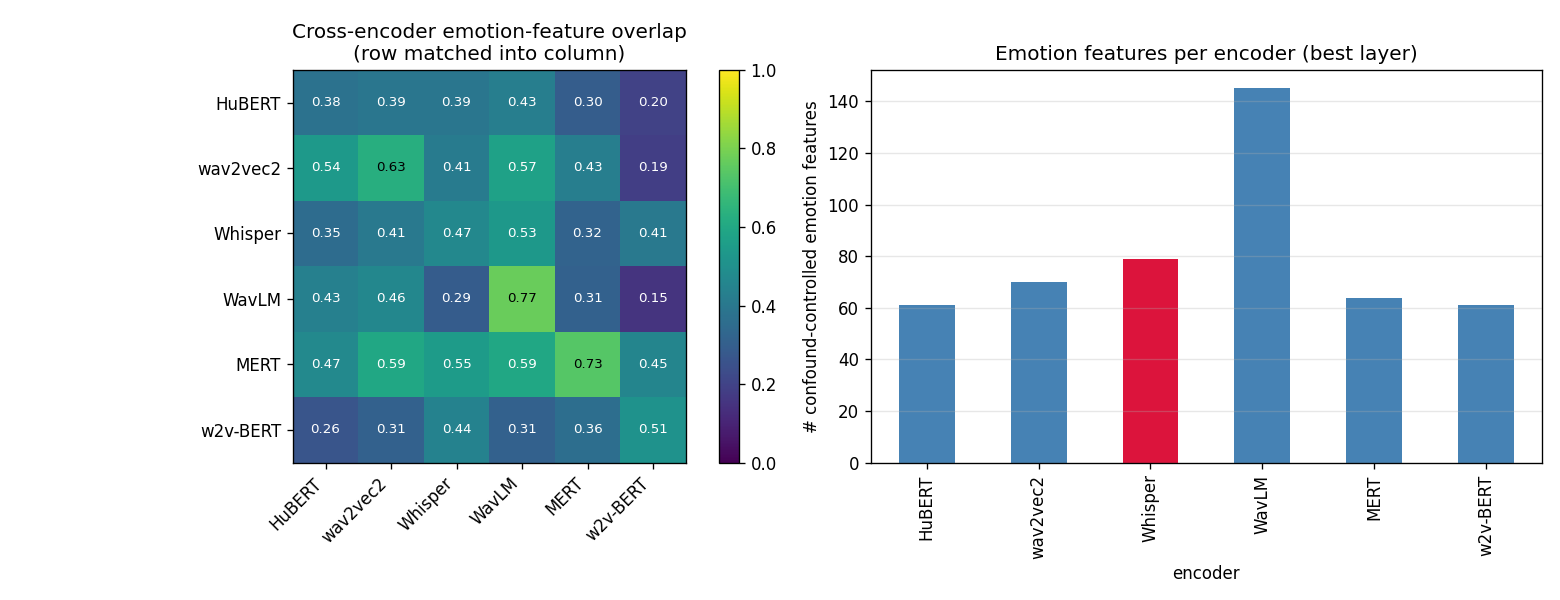
\includegraphics[width=0.96\textwidth]{fig_crossenc.png}
  \caption{Cross-encoder picture. \textbf{Left:} how much each encoder's emotion features overlap with every other's --- Whisper is not an outlier. \textbf{Right:} number of clean emotion features per encoder at its best layer.}
  \label{fig:crossenc}
\end{figure*}

\begin{table}[t]
\caption{Per-encoder emotion features at each encoder's best CREMA-D layer.}
\label{tab:encoders}\small
\begin{tabular}{lccl}
\toprule
Encoder & Best layer & \# emotion feats & Family \\ \midrule
HuBERT   & 13 & 61  & SSL (ASR-style) \\
wav2vec2 & 10 & 70  & SSL (ASR-style) \\
Whisper  & 12 & 79  & Supervised ASR \\
WavLM    & 14 & 145 & SSL (ASR-style) \\
MERT     &  9 & 64  & Music SSL \\
w2v-BERT & 17 & 61  & SSL (multilingual) \\
\bottomrule
\end{tabular}
\end{table}

\begin{table}[t]
\caption{EMIS text-bias (text $-$ audio accuracy) at each encoder's most text-biased layer; positive $=$ takes the lexical shortcut. Raw mean-pooled activations.}
\label{tab:emis}\small
\begin{tabular}{lcc}
\toprule
Encoder & Text-bias & Verdict \\ \midrule
wav2vec2 (L15) & $+0.87$ & takes the shortcut \\
HuBERT (L20)   & $+0.79$ & takes the shortcut \\
WavLM (L20)    & $+0.73$ & takes the shortcut \\
\textbf{Whisper (L24)} & $\mathbf{-0.11}$ & \textbf{resists (voice-grounded)} \\
MERT           & $-0.60$ & resists (music model) \\
w2v-BERT       & $-0.60$ & resists \\
\bottomrule
\end{tabular}
\end{table}

\begin{table}[t]
\caption{Key numbers (HuBERT / CREMA-D, layer 13 unless noted).}
\label{tab:key}\small
\begin{tabular}{ll}
\toprule Quantity & Value \\ \midrule
SAE reconstruction (variance explained) & $93\%$ (FVU 0.07) \\
Dictionary / sparsity / dead features & $8192$ / $k{=}32$ / $4$ \\
Emotion feats: significant $\to$ clean $\to$ confound-OK & $6407 \to 394 \to 61$ \\
Decode peak / disentangle peak / purity peak & L10 / L7 / L2 \\
Acoustic features (positive control) & $60/61$ \\
Decode from acoustic / lexical / random feats & $0.55 / 0.43 / 0.42$ \\
Cross-speaker leave-one-out drop & $\approx 0$ \\
EMIS: Whisper L24 / mean ASR-SSL text-bias & $-0.11 / +0.80$ \\
\bottomrule
\end{tabular}
\end{table}

\section{The pipeline, and what is released}
The study runs as nine numbered, reproducible steps (Table~\ref{tab:pipeline}), each a module under \texttt{src/sae/steps/} callable as \texttt{python -m src.sae.steps <step>}. Heavy jobs (extraction, the 25-layer SAE grid) fan out as SLURM array jobs on a single V100 each. Everything needed to reproduce a number is versioned: the per-step CSVs, plots, and metrics live under \texttt{results/SAE/}; the large activation tensors and SAE checkpoints live on scratch (too big for version control) with pointers recorded. CREMA-D was pulled from a public mirror and EMIS from its open Zenodo release.

\begin{table}[t]
\caption{The pipeline. Each step is one reproducible command.}
\label{tab:pipeline}\small
\begin{tabular}{cll}
\toprule
Step & Does & Headline output \\ \midrule
0 & inventory the cached embeddings & coverage map \\
0.5 & extract per-frame activations & $940$k frames \\
1 & train a TopK SAE & 93\% variance, 4 dead \\
2 & find emotion features (confound-ctrl) & $394\to61$ \\
3 & label acoustic vs.\ lexical & 60/61 acoustic \\
4 & depth sweep (all 25 layers) & L10 vs.\ L7 \\
5 & cross-encoder overlap & Whisper not special \\
6 & cross-speaker (leave-one-out) & drop $\approx 0$ \\
7 & causal sufficiency & $0.55$ vs.\ $0.43$ \\
8 & EMIS text-bias by depth & shortcut is deep \\
\bottomrule
\end{tabular}
\end{table}

\section{Related work and how we differ}
The closest method paper is \emph{AudioSAE}~\cite{audiosae2026} (EACL 2026): the same SAE recipe (TopK, $8\times$, per-frame, all layers) on two encoders, even with a cross-model feature-overlap analysis. But it treats emotion as just one of four generic probe tasks --- no dedicated emotion-feature interpretation, no confound check, no lexicon-controlled corpus, and no acoustic-vs-lexical split. Two further SAE-for-speech papers find phonetic features~\cite{pluth2026asrsae} or singing-technique features~\cite{mariotte2026audioexplain}, not affect, and do not sweep depth. The closest mechanistic SER paper~\cite{ma2026lora} uses probing, logit-lens and CKA but \emph{no} SAEs; the acoustic-vs-lexical question itself is studied with text-dependency analyses~\cite{textdep2024,lexicalser2025} and the EMIS benchmark~\cite{emis2025}. Our specific combination --- confound-controlled emotion features on a lexicon-controlled factorial corpus across six encoders, plus the depth and EMIS results --- is, to our knowledge, new.

\section{Limitations and next steps}
Because emotion is spread across thousands of features, removing a handful barely dents accuracy, so we rely on the \emph{sufficiency} test rather than ablation. One caution we learned the hard way: the SAE's \emph{reconstruction} must not stand in for raw activations in the EMIS probe --- doing so spuriously flips Whisper. Most depth results are on HuBERT/CREMA-D; the cross-encoder and EMIS arms use one layer per encoder rather than full 25-layer grids. Two follow-ups are coded and waiting on data: a causal ablation on IEMOCAP with \emph{real} transcripts, and a SpeechCraft cross-lingual study to explain the published English$\leftrightarrow$Chinese collapse as disjoint feature sets. Beyond those: feature \emph{steering} (turning an emotion feature up to shift predictions) would upgrade our correlational claims to causal ones.

\bibliographystyle{ACM-Reference-Format}
\bibliography{references}
\end{document}
